\section{GUI Implementation}
\subsection{Frameworks}

The most fundamental framework used by the GUI is the Apache Pivot\footnote{\url{http://pivot.apache.org/}}. As authors say, \lq\lq{}Apache Pivot is an open-source platform for building installable Internet applications (IIAs)\rq\rq{}. It is a quite new project, which brings an entirely new approach to building an user interface in Java. The biggest feature of Pivot is the ability to totally decouple the interface description from a programming language. The framework uses the XML markup in the form of BXML files to build interfaces. An example of such a file can be found in Figure~\ref{fig:bxml_example}.

\begin{figure}[ht]
\centering
\begin{Verbatim}[commandchars=\\\{\},frame=single,framerule=0.2pt] 
\PY{n+nt}{<Window} \PY{n+na}{title=}\PY{l+s}{"Hello BXML!"} \PY{n+na}{maximized=}\PY{l+s}{"true"} 
\PY{n+na}{xmlns:bxml=}\PY{l+s}{"http://pivot.apache.org/bxml"} 
\PY{n+na}{xmlns=}\PY{l+s}{"org.apache.pivot.wtk"}\PY{n+nt}{>} 
\PY{n+nt}{<Label} \PY{n+na}{text=}\PY{l+s}{"Hello BXML!"} 
\PY{n+na}{styles=}\PY{l+s}{"\PYZob{}font:'Arial bold 24', color:'#ff0000',} 
\PY{l+s}{ horizontalAlignment:'center', verticalAlignment:'center'\PYZcb{}"}\PY{n+nt}{/>} 
\PY{n+nt}{</Window>} 
\end{Verbatim} 
\caption{Example of BXML syntax}
\label{fig:bxml_example}
\end{figure}

The data binding is another great mechanism of Pivot. It provides own collections, which triggers updates of the UI state, on change of its content and vice versa, updating the state of view components is automatically applied to an underlying data structure. Additionally, it provides means to bind UI items with controller class members. These features simplify the realization of the MVC design pattern a lot. All views in the GUI component are implemented using the BXML syntax and are bound to controllers. What is also worth to mention, Pivot allows to easily internationalize the application, and SemSimMon uses its i18n features - all texts in labels and other UI widgets are internationalized. The default, English localization has been provided.

Another framework that the GUI uses is the well known Spring Framework\footnote{\url{http://www.springsource.org}}. Spring integrates all the components of this module, to associate controllers with views and the model. For this purpose, I use the Inversion of Control Container\footnote{\url{http://static.springsource.org/spring/docs/3.0.x/reference/beans.html}}. 

\subsection{Controller infrastructure}

Controllers are most salient in MVC, and thus need a more attention. There are a few core mechanisms in SemSimMon that needs to be understood to enable work with the GUI module.

All controllers inherit from a common super class, namely the \texttt{BaseController}. This class contains a Pivot component (view) that a given controller manages, a resource (a reference to a bxml file) that must be used to read and instantiate the view and a i18n resource file. The \texttt{BaseController} is responsible for creating a view component from a resource, and bind all widgets and button actions. Additionally, it defines two abstract methods that can be used for fine-tuning of the configuration: \texttt{preDeserialize} and \texttt{postBinding}. The \texttt{preDeserialize} callback is called after Spring initializes the controller, after all dependencies are configured and just before the \texttt{BasicController} tries to deserialize a view. It can be used to initialize resources needed by the deserializer or edit in some other way the resource that will be used for parsing components. The \texttt{BasicController} calls the \texttt{postBinding} method directly after completing the deserialization of the view component. It can be used to initialize UI components or populate some static data.

Binding button actions needs to be described a bit more detailed, as it is a crucial mechanism in the GUI module. It was created with an assumption that most actions in GUI applications are triggered by the user clicking on a button (the \texttt{PushButton} class in Pivot). To reduce a boilerplate code that needs to be written to handle a single action, I have designed a \texttt{ButtonAction} mechanism. It is composed of the \texttt{BasicController} that binds actions to methods, the \texttt{@ButtonAction} annotation that can be used to mark a method which should be called on a button click, and finally the \texttt{ReflectionButtonPressListener} class, which is responsible for processing a given method. To handle an action request submitted by the user, developer needs to do three things: define a push button with an appropriate id in view; define a class member of the \texttt{PushButton} type and of the same name as the id defined in the view; and finally declare a method in the controller and mark it using the \texttt{@ButtonAction} annotation.

Giving on an example is the best way, to show how the MVC pattern works in the SemSimMon. Let us assume that we need a basic view, composed of one panel with a single label and a button. On a button click, the label gets filled with a random content. The first thing that needs to be done is to define a view using the BXML notation. This example view can be found in Figure~\ref{fig:sample_view}.

\begin{figure}[ht]
\centering
\begin{Verbatim}[commandchars=\\\{\},frame=single,framerule=0.2pt] 
\PY{c+cp}{<?xml version="1.0"?>}
\PY{n+nt}{<BoxPane} \PY{n+na}{xmlns:bxml=}\PY{l+s}{"http://pivot.apache.org/bxml"}
\PY{n+na}{xmlns=}\PY{l+s}{"org.apache.pivot.wtk"} \PY{n+na}{orientation=}\PY{l+s}{"vertical"}\PY{n+nt}{>}
\PY{n+nt}{<Label} \PY{n+na}{bxml:id=}\PY{l+s}{"label"} \PY{n+na}{text=}\PY{l+s}{"%sample.label"}\PY{n+nt}{/>}
\PY{n+nt}{<PushButton} \PY{n+na}{bxml:id=}\PY{l+s}{"generateButton"}
\PY{n+na}{buttonData=}\PY{l+s}{"%sample.generate"}\PY{n+nt}{/>}
\PY{n+nt}{</BoxPane>}
\end{Verbatim} 
\caption{The definition of an example UI component, written in the BXML notation.}
\label{fig:sample_view}
\end{figure}

This view consists of only three items: a box pane, with vertical orientation, and inside of it: a label and a push button. What should be additionally noticed is that the texts of labels and buttons are internationalized. In Pivot, i18n keys are stored in JSON\footnote{JSON stands for(JavaScript Object Notation, see \url{http://www.json.org/}} files. Figure~\ref{fig:i18n} covers the content of an example JSON file that is a valid Pivot i18n resource. 

\begin{figure}[ht]
\centering
\begin{Verbatim}[commandchars=\\\{\},frame=single,framerule=0.2pt] 
\PY{p}{\PYZob{}}
\PY{l+s+s2}{"sample"} \PY{o}{:} \PY{p}{\PYZob{}}
\PY{l+s+s2}{"label"} \PY{o}{:} \PY{l+s+s2}{"Sample content of label"}\PY{p}{,}
\PY{l+s+s2}{"generate"} \PY{o}{:} \PY{l+s+s2}{"Generate text!"}
\PY{p}{\PYZcb{}}
\PY{p}{\PYZcb{}}
\end{Verbatim} 
\caption{Sample internationalization bundle}
\label{fig:i18n}
\end{figure}

A next thing to do is to create a \texttt{SampleController}. It will contain a label, a button and 2 handler methods, to show that one button may trigger multiple methods, which can be called either on a UI thread (Event Dispatching Thread) or as a background task. Figure~\ref{fig:sample_controller} shows a listing of the \texttt{SampleController} class implementation.

\begin{figure}[ht]
\centering
\begin{Verbatim}[commandchars=\\\{\},numbers=left,firstnumber=1,stepnumber=1]
\PY{k+kn}{package} \PY{n}{pl}\PY{o}{.}\PY{n+na}{edu}\PY{o}{.}\PY{n+na}{agh}\PY{o}{.}\PY{n+na}{semsimmon}\PY{o}{.}\PY{n+na}{gui}\PY{o}{.}\PY{n+na}{controllers}\PY{o}{;}

\PY{k+kn}{import} \PY{n+nn}{org.apache.pivot.beans.BXML}\PY{o}{;}
\PY{k+kn}{import} \PY{n+nn}{org.apache.pivot.wtk.BoxPane}\PY{o}{;}
\PY{k+kn}{import} \PY{n+nn}{org.apache.pivot.wtk.Label}\PY{o}{;}
\PY{k+kn}{import} \PY{n+nn}{org.apache.pivot.wtk.PushButton}\PY{o}{;}
\PY{k+kn}{import} \PY{n+nn}{org.slf4j.Logger}\PY{o}{;}
\PY{k+kn}{import} \PY{n+nn}{org.slf4j.LoggerFactory}\PY{o}{;}
\PY{k+kn}{import} \PY{n+nn}{pl.edu.agh.semsimmon.gui.controllers.action.ButtonAction}\PY{o}{;}

\PY{k+kd}{public} \PY{k+kd}{class} \PY{n+nc}{SampleController} \PY{k+kd}{extends} \PY{n+nc}{BaseController}\PY{o}{<}\PY{n+nc}{BoxPane}\PY{o}{>} \PY{o}{\PYZob{}}

  \PY{k+kd}{public} \PY{k+kd}{static} \PY{k+kd}{final} \PY{n}{Logger} \PY{n}{log} \PY{o}{=} \PY{n}{LoggerFactory}\PY{o}{.}\PY{n+na}{getLogger}\PY{o}{(}\PY{n}{SampleController}\PY{o}{.}\PY{n+na}{class}\PY{o}{)}\PY{o}{;}

  \PY{n+nd}{@BXML}
  \PY{k+kd}{private} \PY{n}{PushButton} \PY{n}{generateButton}\PY{o}{;}

  \PY{n+nd}{@BXML}
  \PY{k+kd}{private} \PY{n}{Label} \PY{n}{label}\PY{o}{;}

  \PY{k+kd}{private} \PY{k+kt}{int} \PY{n}{i} \PY{o}{=} \PY{l+m+mi}{0}\PY{o}{;}

  \PY{n+nd}{@ButtonAction}\PY{o}{(}\PY{n}{type} \PY{o}{=} \PY{n}{ButtonAction}\PY{o}{.}\PY{n+na}{Type}\PY{o}{.}\PY{n+na}{INSTANT}\PY{o}{)}
  \PY{k+kd}{private} \PY{k+kt}{void} \PY{n+nf}{cancelButtonPressed}\PY{o}{(}\PY{o}{)} \PY{o}{\PYZob{}}
    \PY{n}{label}\PY{o}{.}\PY{n+na}{setText}\PY{o}{(}\PY{l+s}{"Sample content "} \PY{o}{+} \PY{n}{i}\PY{o}{+}\PY{o}{+}\PY{o}{)}\PY{o}{;}
  \PY{o}{\PYZcb{}}

  \PY{n+nd}{@ButtonAction}\PY{o}{(}\PY{n}{target} \PY{o}{=} \PY{l+s}{"cancelButton"}\PY{o}{,} \PY{n}{type} \PY{o}{=} \PY{n}{ButtonAction}\PY{o}{.}\PY{n+na}{Type}\PY{o}{.}\PY{n+na}{BACKGROUND}\PY{o}{)}
  \PY{k+kd}{private} \PY{k+kt}{void} \PY{n+nf}{backgroundTaskOfGenerateButton}\PY{o}{(}\PY{o}{)} \PY{k+kd}{throws}
\PY{n}{InterruptedException} \PY{o}{\PYZob{}}
    \PY{n}{log}\PY{o}{.}\PY{n+na}{debug}\PY{o}{(}\PY{l+s}{"Starting background task"}\PY{o}{)}\PY{o}{;}
    \PY{n}{Thread}\PY{o}{.}\PY{n+na}{sleep}\PY{o}{(}\PY{l+m+mi}{5000}\PY{o}{)}\PY{o}{;}
    \PY{n}{log}\PY{o}{.}\PY{n+na}{debug}\PY{o}{(}\PY{l+s}{"Background task done"}\PY{o}{)}\PY{o}{;}
  \PY{o}{\PYZcb{}}

  \PY{n+nd}{@Override}
  \PY{k+kd}{protected} \PY{n}{Class} \PY{n+nf}{getBindableClass}\PY{o}{(}\PY{o}{)} \PY{o}{\PYZob{}}
    \PY{k}{return} \PY{n}{SampleController}\PY{o}{.}\PY{n+na}{class}\PY{o}{;}
  \PY{o}{\PYZcb{}}
\PY{o}{\PYZcb{}}
\end{Verbatim}
 
\caption{Listing of SampleController.java}
\label{fig:sample_controller}
\end{figure} 

In the line 12 of SampleController.java, we can see a class definition. The \texttt{BaseController} is a class template and takes the class of pivot component as a specification parameter. In this case, it is the \texttt{BoxPane} class. The Next noteworthy lines are 15-16 and 18-19. These lines contain a declaration of UI widgets that will be bound from the view. In oder to bind to a view\rq{}s UI widget to given controller\rq{}s class attribute, the attribute must be marked using the \texttt{@BXML} annotation and must have a name same as the \texttt{bxml:id} property of the widget. This class defines two handlers that are triggered by a click on \texttt{generateButton}.

The final step is to associate all these items each other, using Spring xml configuration. Such a configuration can be found in Figure~\ref{fig:sample_spring}.

\begin{figure}[ht]
\centering
\begin{Verbatim}[commandchars=\\\{\},frame=single,framerule=0.2pt]
\PY{c+cp}{<?xml version="1.0" encoding="UTF-8"?>}
\PY{n+nt}{<beans}
  \PY{n+nt}{<bean} \PY{n+na}{id=}\PY{l+s}{"sampleController"} 
        \PY{n+na}{class=}\PY{l+s}{"pl.edu.agh.semsimmon.gui.controllers.SampleController"}
        \PY{n+na}{parent=}\PY{l+s}{"baseController"}\PY{n+nt}{>}
    \PY{n+nt}{<property} \PY{n+na}{name=}\PY{l+s}{"bxmlContentResource"} \PY{n+na}{value=}\PY{l+s}{"classpath:ui/sample.bxml"}\PY{n+nt}{/>}
    \PY{n+nt}{<property} \PY{n+na}{name=}\PY{l+s}{"listenerFactory"} \PY{n+na}{ref=}\PY{l+s}{"buttonPressListenerFactory"}\PY{n+nt}{/>}
    \PY{c}{<!--}\PY{c}{ Dependencies to model should go here}\PY{c}{-->}
  \PY{n+nt}{</bean>}
\PY{n+nt}{</beans>}
\end{Verbatim}
 
\caption{Listing of a sample Spring configuration}
\label{fig:sample_spring}
\end{figure}

\subsection{Visualization types}

As stated in the requirements analysis, the system will provide the user with an option to use 4 plot types: \emph{time series} plot, \emph{pie chart}, \emph{bar chart} and so called \emph{spider web chart}. Figures~\ref{fig:spider_sample}~\ref{fig:piechart_example},~\ref{fig:barchart_example}~and~\ref{fig:piechart_example} depict example screen shots of each visualization type supported by SemSimMon. The spider web chart is the most interesting one, as it allows to have a quick overview of a resources misuse in the context of multiple capabilities. Figure~\ref{fig:spider_sample} covers an example screen shot of this plot type. The plot contains the heap and non heap memory usage of 3 JVM instances.


\begin{figure}[ht]
\centering
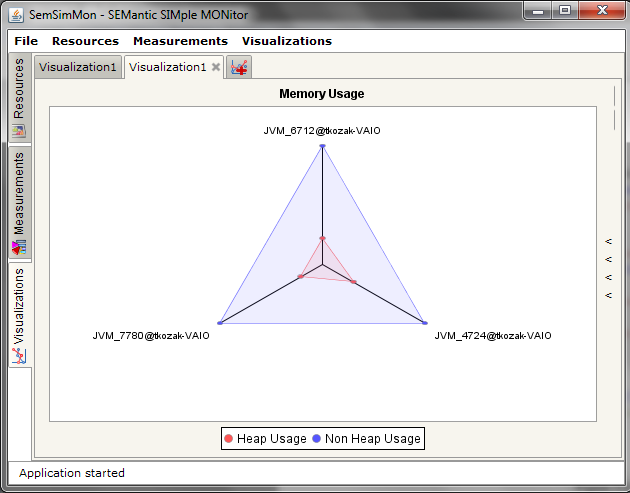
\includegraphics[width=0.8\textwidth]{spider_sample}
\caption{Spider web display}
\label{fig:spider_sample}
\end{figure}
\clearpage
\begin{figure}[ht]
\centering
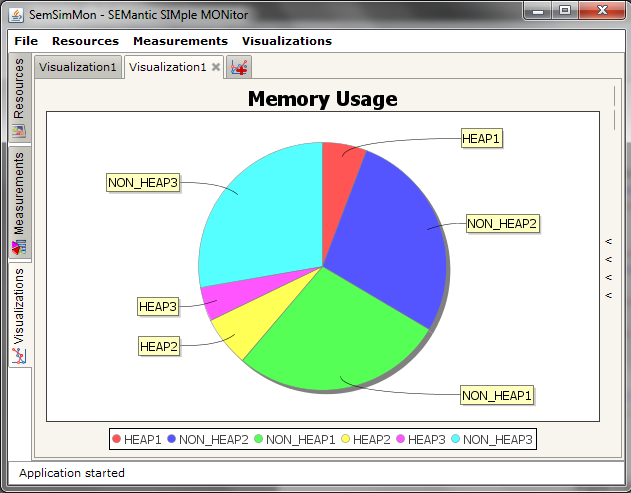
\includegraphics[width=0.6\textwidth]{piechart_example}
\caption{Pie chart.}
\label{fig:piechart_example}
\end{figure}

\begin{figure}[ht]
\centering
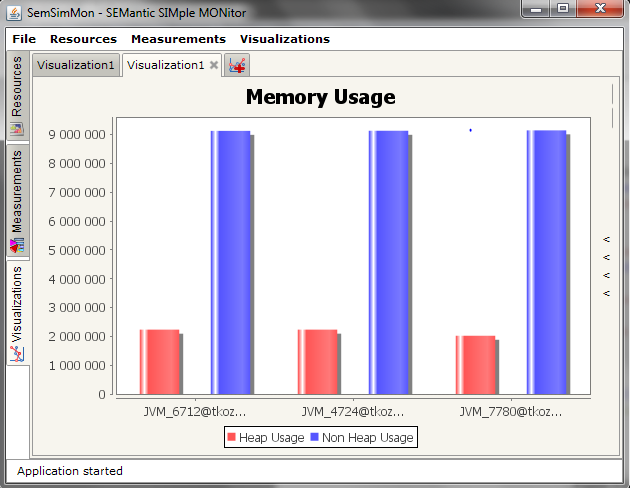
\includegraphics[width=0.6\textwidth]{barchart_example}
\caption{Bar graph.}
\label{fig:barchart_example}
\end{figure}
\clearpage
\begin{figure}[ht]
\centering
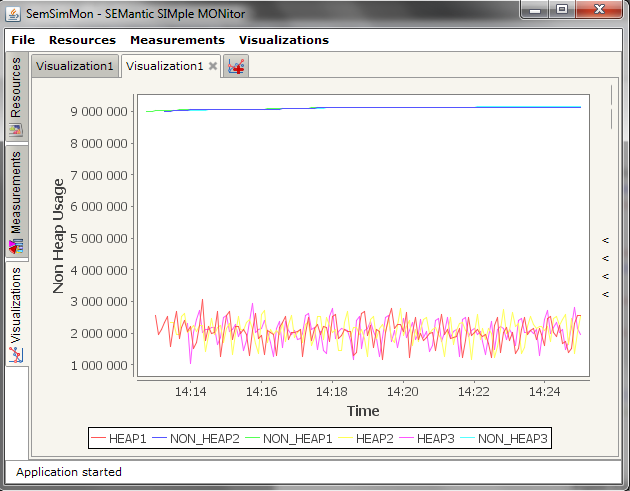
\includegraphics[width=0.7\textwidth]{time_series_example}
\caption{Time series plot (multicurve.}
\label{fig:piechart_example}
\end{figure}